\documentclass{UoNMCHA}
\usepackage[authoryear]{natbib}
\usepackage{array,booktabs} % For nice tables
\usepackage{amsmath,amsfonts,amssymb} % For nice maths
\usepackage{color}
\usepackage{multicol}
\usepackage{enumerate}
\usepackage{listings}
\usepackage{subfig}
\usepackage{hyperref}
\usepackage[parfill]{parskip}   % For replacing paragraph indenting with a newline instead
\newif\ifcomment
\commenttrue
\commentfalse
% Number equations per section
\numberwithin{equation}{section}

\hypersetup{
%    bookmarks=true,         % show bookmarks bar?
%    unicode=false,          % non-Latin characters in AcrobatÕs bookmarks
%    pdftoolbar=true,        % show AcrobatÕs toolbar?
%    pdfmenubar=true,        % show AcrobatÕs menu?
%    pdffitwindow=false,     % window fit to page when opened
%    pdfstartview={FitH},    % fits the width of the page to the window
%    pdftitle={My title},    % title
%    pdfauthor={Author},     % author
%    pdfsubject={Subject},   % subject of the document
%    pdfcreator={Creator},   % creator of the document
%    pdfproducer={Producer}, % producer of the document
%    pdfkeywords={keyword1} {key2} {key3}, % list of keywords
%    pdfnewwindow=true,      % links in new window
    colorlinks=true,       % false: boxed links; true: colored links
    linkcolor=blue,          % color of internal links
    citecolor=blue,        % color of links to bibliography
%    filecolor=magenta,      % color of file links
    urlcolor=blue           % color of external links
}

\definecolor{light-gray}{gray}{0.95}
\definecolor{myblue}{RGB}{20,105,176}
\definecolor{myorange}{RGB}{255,140,0}
\definecolor{mygrey}{RGB}{64,64,64}
\definecolor{MATLABKeyword}{rgb}{0,0,1}
\definecolor{MATLABComment}{rgb}{0.1328125,0.54296875,0.1328125}
\definecolor{MATLABString}{rgb}{0.625,0.125,0.9375}

\lstset{language=Matlab,
    basicstyle=\small\ttfamily,
    keywordstyle=\color{MATLABKeyword},
    %identifierstyle=,
    commentstyle=\color{MATLABComment},
    stringstyle=\color{MATLABString},
    numberstyle=\tiny,
    %numbers=left,
    basewidth=0.5em}
\lstset{
language=C,
numbers=none,
xleftmargin=1cm,
frame=tblr,
classoffset=0,
morekeywords={r0,r1,r2,r3,r4,r5,r6,r7,r8,r9,r10,r11,r12,r13,r14,r15},keywordstyle=\color{myblue},
classoffset=1,
morekeywords={ldr,srt,sub,cmp,it,bgt,b,str,beq},	keywordstyle=\color{myorange},
classoffset=0,
commentstyle=\color{MATLABComment},
breaklines=true,
postbreak=\space //...
}

\firstpage{1}    % Set page number for first page
\UoNMCHAreportNo{ELEC1710  } %Report number
\UoNMCHAyear{ }   % Year
\shorttitle{ELEC1710 - Lab 1} %For odd pages
%%%%%%%%%%%%%%%%%%%%%%%%%%%%%%%%%%%%%%%%%%%%%%%%%%%%
\begin{document}
\title{Lab 6:\\Fundamentals of Assembly Language Part 2: \\ Flow Control and Arithmetic \\ \ \\
{\small ELEC1710   \\ 
}}
%\author[UoNMCHA]{Student Name}
%\address[UoNMCHA]{
%Student of Mechatronics Engineering,\\
%The University of Newcastle, Callaghan, NSW 2308, AUSTRALIA \\
%Student Number: 3...... \\
%E-mail: \href{mailto:First.Last@uon.edu.au}{\textsf{First.Last@uon.edu.au}}}
%%%%%%%%%%%%%%%%%%%%%%%%%%%%%%%%%%%
\maketitle
\onecolumn

\vspace{-5mm}

\section{Introduction}

This programming task demonstrates the basic use of arithmetic and flow control instructions in Thumb assembly. Conditional execution will be introduced by modifying Lab 4's \texttt{blinky} example so that the blinking can be controlled with an external push button. Arithmetic instructions will then be used to implement a basic \texttt{for} loop which will cause the LED to only flash a set number of times.

\section{Assembly Reference}

\subsection{Arithmetic: \texttt{add} and \texttt{sub}}

The arithmetic instructions \texttt{add} and \texttt{sub} can be used in several different ways. The general syntax is as follows:

\texttt{add\{s\}\{cond\} \{Rd,\} Rn, Operand2} \\
\texttt{sub\{s\}\{cond\} \{Rd,\} Rn, Operand2}

where:

\begin{itemize}
    \item \texttt{s} optionally updates the condition flags in \texttt{APSR}. \textbf{NB:} This is required when using conditional execution.
    \item \texttt{cond} is a conditional execution suffix from Figure \ref{fig:cond}.
    \item \texttt{Rd} is an optional destination register. If not specified the result overwrites \texttt{Rn}.
    \item \texttt{Rn} is the first operand.
    \item \texttt{Operand2} is the second operand and can be a constant preceeded by a \# symbol (eg \#14), another register, or another register with bit shift.
\end{itemize}

The most basic usage is to add or subtract a constant, for example:

\texttt{add r2, \#143 \quad // r2 = r2 + 143} \\
\texttt{sub r1, \#4 \quad //r1 = r1 - 4}

Using this syntax the constant can be any value in the range 0-4095 (ie: it is encoded as a 12-bit unsigned binary number).

It is possible for the destination register to differ from the source, for example:

\texttt{add r1, r2, \#4 \quad // r1 = r2 + 4}

or for the 12-bit constant to be replaced with a register:

\texttt{add r1, r2, r5 \quad // r1 = r2 + r5}.

In its most complicated form the last operand can also include a shift, for example:

\texttt{add r2, r3, r4, LSL \#2 \quad // r2 = r3 + (r4 << 2) = r2 = r2 + 4*r4}

\begin{figure}[h!]
\makebox[\textwidth][c]{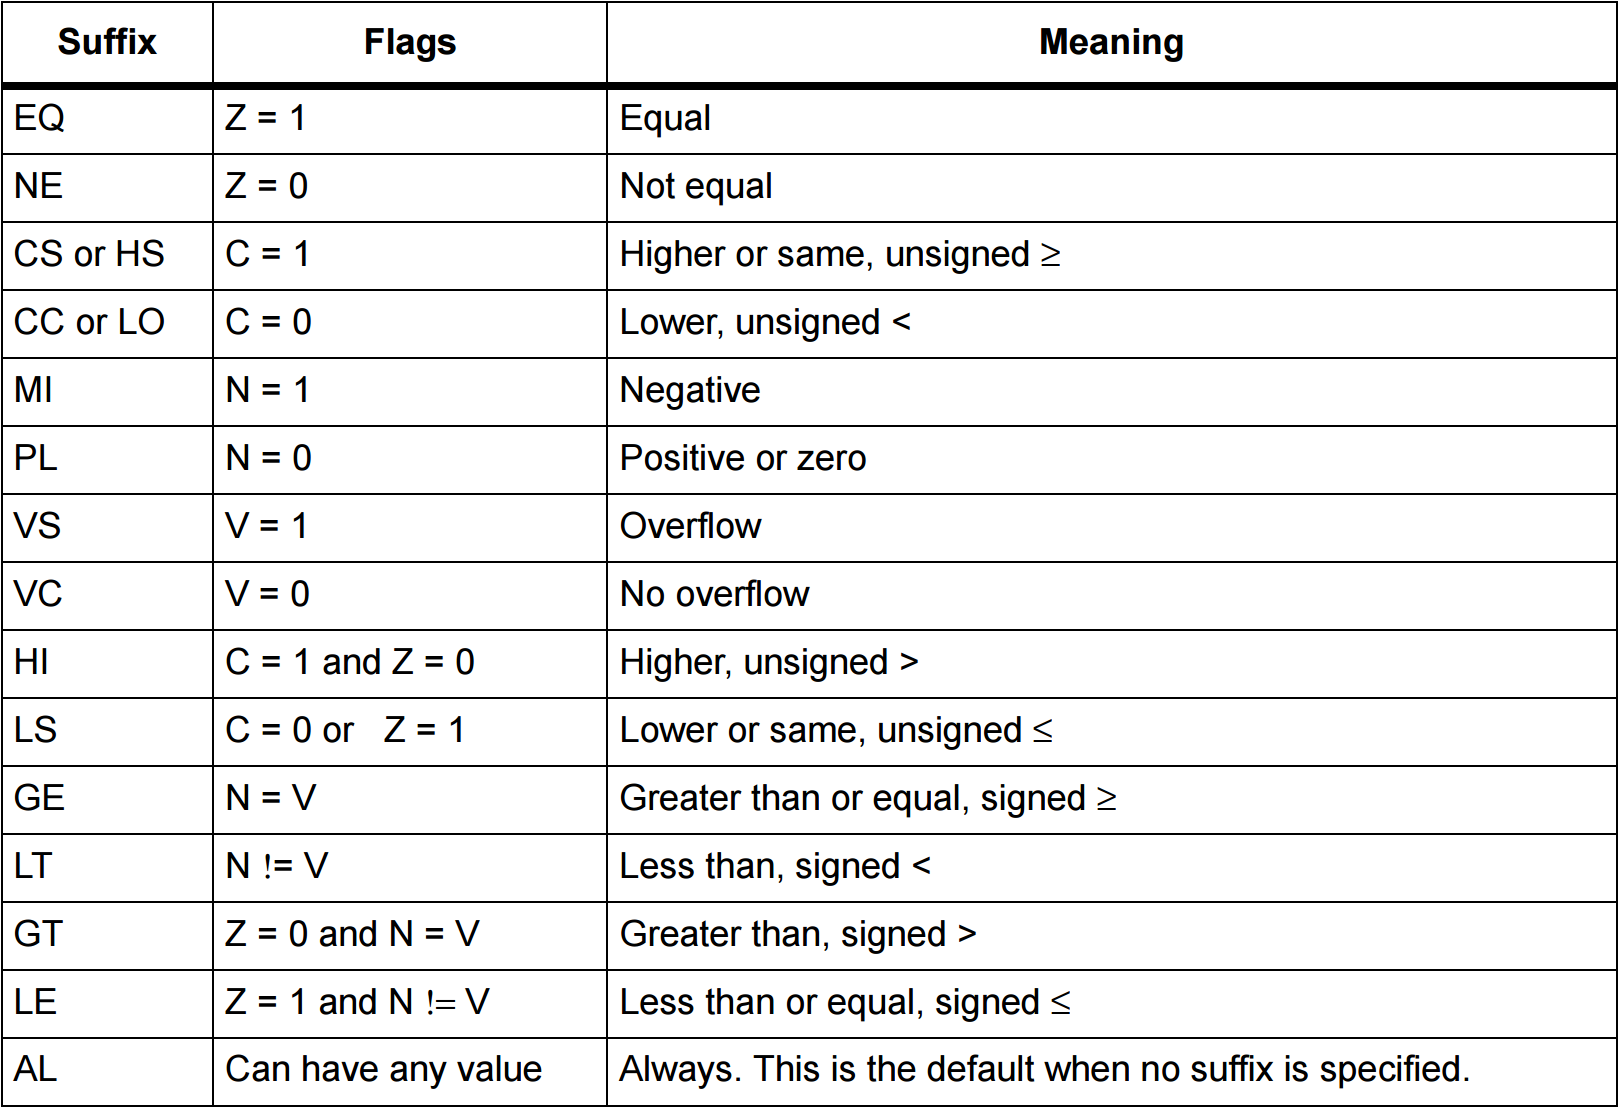
\includegraphics[width=0.7\textwidth]{Figures/cond}}
\caption{Condition code suffixes, extracted from \textit{The Cortex-M3 Instruction Set}, ST-Microelectronics document number PM0056.}
\label{fig:cond}
\end{figure}


\subsection{Comparison: \texttt{cmp} and \texttt{cmn}}

The comparison instructions set the conditions flags in \texttt{APSR} based on the sum or difference between two values. They are the equivalent to performing an \texttt{adds} or \texttt{subs} instruction except the result of the calculation is discarded. As such comparison instructions are more register efficient than arithmetic instructions.

The syntax is as follows:

\texttt{cmp\{cond\} Rn, Operand2 \\ cmn\{cond\} Rn, Operand2}

Where \texttt{Rn} must be a register and \texttt{Operand2} can be a constant, register, or register with bit shift.

The \texttt{cmp} sets condition flags from the result of \texttt{Rn - Operand2} while \texttt{cmn} performs \texttt{Rn + Operand2} and sets flags.

A full list of condition suffixes and associated \texttt{APSR} flags can be found in Figure \ref{fig:cond}.

Usage example:

\begin{lstlisting}[
caption = Example of the \texttt{cmp} instruction.,
label = 
]
ldr r1, = 0x100
cmp r1, #0x100  // Results in Z = 1, EQ, LS and LE conditions become true
\end{lstlisting}

\subsection{Branch: \texttt{b}}

The \texttt{b} instruction causes program execution to jump to a location specified by an assembly label. The syntax useful for this lab is:

\texttt{b\{cond\} label}

Where \texttt{label} is an ASCII string followed by a `:' character in the assembly listing and \texttt{cond} is a condition suffix from Figure \ref{fig:cond}.

Example:

\begin{lstlisting}[
caption = Example of the \texttt{b} instruction.,
label = 
]
start:
    // Useful code goes in here

    b start     // Jump back to "start" to form an infinite loop
\end{lstlisting}

\subsection{If-Then: \texttt{it}}

In Thumb assembly all instructions using a conditional execution suffix must be preceded by an \texttt{it} instruction. Up to four instructions can be included in this block however only basic usage will be documented here.

The full syntax is:

\texttt{it\{x\{y\{z\}\}\} cond}

Where \texttt{x},\texttt{y} and \texttt{z} specify the condition for the optional 2nd, 3rd and 4th instructions and are either \texttt{t} (then, execute if \texttt{cond} is met) or \texttt{e} (else, execute if \texttt{cond} is NOT met). The \texttt{cond} suffix is one of those listed in Figure \ref{fig:cond}.

Simple examples of the \texttt{it} instruction are shown in Listings \ref{lst:if} and \ref{lst:for}. More advanced usage requiring multiple instructions should not be required for this lab.

\vspace{7cm}

\pagebreak

\section{Code Examples}

\begin{lstlisting}[
caption = \texttt{if()} statement example in Thumb assembly.,
label = lst:if
]
// if(r1 == 5)

	cmp r1, #5	// Compare r1 and the decimal constant 5, sets status bits
	it eq		// If-Then block testing equal-to status
	beq iseq	// branch to 'iseq' if status bits matched equal to
	b isnoteq	// Unconditional branch (ie: GOTO) 'isnoteq'

iseq: 
	// Code executed if r1 is equal to 5

isnoteq:
\end{lstlisting}

\begin{lstlisting}[
caption = \texttt{for()} loop example in Thumb assembly,
label = lst:for
]
// for(x = 0x80000; x > 0; x--) { loop_code() }

    ldr r3, =0x00080000 // This function counts down from this number
testExit:               // Label addressing start of loop
    sub r3, r3, #1      // Subtract 1 from r3 and store result back in r3
    cmp r3, #0          // Compare r3 to zero. This sets status flags
    it gt               // IT (if-then) block with greater than condition
    bgt do_loop         // If the comparison result (ie: the status flags)
    b exitLoop          // Unconditional branch to 'exitLoop',
                        // this occurs if the branch to 'do_loop' failed
do_loop:
    // write loop_code() here
    b testExit          // After doing stuff test the exit condition

exitLoop:
    // The rest of your program
\end{lstlisting}

\section{Lab Task}

\begin{enumerate}
    \item Construct a single push button with pull-down resistor and connect it to \texttt{GPIOA 0} (pin \texttt{A0} on the development board).
    \item Modify \texttt{main.c} so that it calls \texttt{blinky}. If your code does not compile or is otherwise corrupted you can begin this lab by re-extracting the working template from Lab 4.
    \item Modify constants in \texttt{blinky.s} to increase the blink rate to approximately 2-3Hz. Maintain the 50\% duty cycle.
    \item Add code at the start of \texttt{blinky} which reads the status of \texttt{GPIOA} into a register. Using \texttt{cmp} and \texttt{it} instructions implement an \texttt{if} statement such that the LED only blinks when the external push button is pressed.
    \item Build a \texttt{for} loop around the LED blinking code so that when the button is pushed it causes the LED to flash on/off 10 times then remains off until the button is pushed again.
\end{enumerate}

\end{document}
